%%%%%%%%%%%%%%%%%%%%%%%%%%%%%%%%%%%%%%%%%%%%%%%%%%%%%%%%%%%%%%%%%%%%%%%%%%%%%%%%%%%%%%%%%%%%%%%%%%%%%%%%%%%%%%%%%%%%%%%%%%
% Project Report/Thesis LaTeX Template
%
% Original authors:
% Steven Gunn 
% http://users.ecs.soton.ac.uk/srg/softwaretools/document/templates/
% and
% Sunil Patel
% http://www.sunilpatel.co.uk/thesis-template/
%
% Modified by
% Venkataswamy R, 
% www.venkataswamy.in
%
%%%%%%%%%%%%%%%%%%%%%%%%%%%%%%%%%%%%%%%%%%%%%%%%%%%%%%%%%%%%%%%%%%%%%%%%%%%%%%%%%%%%%%%%%%%%%%%%%%%%%%%%%%%%%%%%%%%%%%%%%%

% Modification and Version

%  Version Number			Date			Author				Modification		
% ------------------------------------------------------------------------------------------------------------------------
%
%  1					22.03.2017			Venkataswamy R		Initial version
%  1.1					23.03.2018			Venkataswamy R		New logo added, Typo error, acknowledgement
%


% Do not modify this file
% Goto Generics/ProjectVariable.tex file and do the modification

%----------------------------------------------------------------------------------------
%	PACKAGES AND OTHER DOCUMENT CONFIGURATIONS
%----------------------------------------------------------------------------------------

\documentclass[12pt, oneside]{Thesis} % The default font size and one-sided printing (no margin offsets)

\graphicspath{{Pictures/}} % Specifies the directory where pictures are stored

\usepackage[square, numbers, comma, sort&compress]{natbib} % Use the natbib reference package - read up on this to edit the reference style; if you want text (e.g. Smith et al., 2012) for the in-text references (instead of numbers), remove 'numbers' 
\hypersetup{urlcolor=blue, colorlinks=true} % Colors hyperlinks in blue - change to black if annoying
\title{\ttitle} % Defines the thesis title - don't touch this

\usepackage{mathptmx, imakeidx,tfrupee, hyperref,listings,color,textcomp,algorithm, pdfpages, setspace,imakeidx, datetime, ragged2e, enumitem}

%\usepackage{fontspec}   Compile with XeLaTeX or LuaLaTeX
%\setmainfont{Times New Roman}

\makeindex

\hypersetup{%
	colorlinks=true,% Colour links without boxes
	linkcolor=black}% Internal link colour is black

\usepackage[noend]{algpseudocode}% http://ctan.org/pkg/algorithmicx
\algrenewcommand\Return{\State \algorithmicreturn{} }%


\definecolor{listinggray}{gray}{0.9}
\definecolor{lbcolor}{rgb}{0.9,0.9,0.9}
\lstset{
	backgroundcolor=\color{lbcolor},
	tabsize=4,
	rulecolor=,
	language=matlab,
	basicstyle=\scriptsize,
	upquote=true,
	aboveskip={1.5\baselineskip},
	columns=fixed,
	showstringspaces=false,
	extendedchars=true,
	breaklines=true,
	prebreak = \raisebox{0ex}[0ex][0ex]{\ensuremath{\hookleftarrow}},
	frame=single,
	showtabs=false,
	showspaces=false,
	showstringspaces=false,
	identifierstyle=\ttfamily,
	keywordstyle=\color[rgb]{0,0,1},
	commentstyle=\color[rgb]{0.133,0.545,0.133},
	stringstyle=\color[rgb]{0.627,0.126,0.941},
}

\makeindex[intoc]

%\usepackage{draftwatermark}
%\SetWatermarkText{Sample}




\begin{document}
	
% All the Variable should be entered inside {}
% If not applicablt leave empty {} do not delete {}.

% Name of the University
\newcommand{\UniversityName}
{CHRIST (Deemed to be University)}


% Title of the project or thesis
\newcommand{\ProjectTitle}
{TITTLE OF PROJECT}

\newcommand{\ProjectTitleTwo}
{Tittle of Project}


% Type of Dissertation M.Tech Dissertation or B.Tech Dissertation
\newcommand{\DissertationType}
{A Project Report on}

% Program name: MASTER OF TECHNOLOGY or BACHELOR OF TECHNOLOGY in Uppercase
\newcommand{\ProgramNameUpper}
{BACHELOR OF TECHNOLOGY}

% Program name: Master of Technology or Bachelor of Technology in Normal case
\newcommand{\ProgramName}
{Bachelor of Technology}

% Program Short form: M.Tech. or B.Tech.
\newcommand{\ProgramNameShort}
{B.Tech.}


% Specialization: 
% For B.Tech : Electrical and Electronics Engineering, Mechanical Engineering 
% For M.Tech : Power Systems, VLSI Design, Software Engineering
\newcommand{\SpecializationName}
{Name of Specialization}


% Name of Student in the Alphabetical Order should be writen in {} for each. Leave blank braces for other Author name if it is individual project
% 
\newcommand{\AuthorNameOne}
{Name 1}

\newcommand{\RegisterNoOne}
{Register No 1}

\newcommand{\AuthorDepartmentOne}
{Electrical \& Electronics Engineering}


\newcommand{\AuthorNameTwo}
{Name 2}

\newcommand{\RegisterNoTwo}
{Register No 2}

\newcommand{\AuthorDepartmentTwo}
{Mechanical Engineering}


\newcommand{\AuthorNameThree}
{Name 3}

\newcommand{\RegisterNoThree}
{Register No 3}

\newcommand{\AuthorDepartmentThree}
{Mechanical Engineering}


\newcommand{\AuthorNameFour}
{Name 4}

\newcommand{\RegisterNoFour}
{Register No 4}

\newcommand{\AuthorDepartmentFour}
{Civil Engineering}


% Name of the Guide
\newcommand{\GuideName}
{Guide Name}

% Designation of the Guide
\newcommand{\GuideDesignation}
{Guide Designation}

% Department of Guide where he belongs to
\newcommand{\GuideDepartment}
{Guide Department}


% Name of the Co-Guide
\newcommand{\CoGuideName}
{Co-Guide Name}

% Designation of the Co-Guide
\newcommand{\CoGuideDesignation}
{Co-Guide Designation}

% Department of Co-Guide where he belongs to
\newcommand{\CoGuideDepartment}
{Co-Guide Department}


\newcommand{\NameofAuthortobeCertified}
{Name 2}

% Leave blank in {} if co-guide is not there or if c0-guide is there then ~and~ in {}
\newcommand{\CoGuideAnd}
{~and~}


% Address of the department where project offically executed
\newcommand{\DepartmentNameAddress}
{ %\renewcommand{\baselinestretch}{1.0}
\textbf{\large{
	Department Name\\ 
	\CollegeName,~ \UniversityName,\\ 
	Kumbalagudu,\,Bengaluru\,-\,560~074
}}

} 


% Project Date in month-yyyy format
\newcommand{\ProjectDate}
{November-2015}

% Academic Year in yyyy-yyyy format
\newcommand{\AcademicYear}
{2015-2016}

% Name of the department only
\newcommand{\DepartmentName}
{Department Name}

% Name of the College
\newcommand{\CollegeName}
{Faculty of Engineering}


% Name of the HOD or Coordinator
\newcommand{\HODorCoordinator}
{Name of the HOD or Coordinator}

% Name of the Position of the Head. eg: Head of the Department, Coordinator
\newcommand{\HODorCoordinatorDesignation}
{Name of the Position of the Head}


% Name of the Vice-Chancellor
\newcommand{\VCName}
{Dr. Rev. Fr. Thomas C Mathew}

% Name of the Pro Vice Chancellor
\newcommand{\ProVCName}
{Dr. Rev. Fr. Abraham}

% Name of the Director of the College
\newcommand{\DirectorName}
{Fr. Benny Thomas}

% Name of the Dean/Associate Dean
\newcommand{\DeanName}
{Dr. Iven Jose}

% Name of the Position of Dean/Associate Dean
\newcommand{\DeanDesignation}
{Associate Dean}


% If the project work done by more than one student then 'We' in side {} or 'I' if individual project 
\newcommand{\WeorI}
{We}

% Acknowledgement for Guide
\newcommand{\AcknowledgementForGuide}
{
	\WeorI~also extremely grateful to my guide, \textbf{\GuideName}, who has supported and helped to carry out the project. His constant monitoring and encouragement helped me keep up to the project schedule.
}

% Acknowledgement for Co-Guide(Leave blank if no co-guide) 
\newcommand{\AcknowledgementForCoGuide}
{
	\WeorI~also extremely grateful to my co-guide, \textbf{\CoGuideName}, who has supported and helped to carry out the project. His constant monitoring and encouragement helped me keep up to the project schedule.
}


% Acknowledgement for Others
\newcommand{\AcknowledgementForOthers}
{
	If outside the college-mention the organisation and the concerned people, like head of the organisation, guide and any other person you want to thank. All faculty and non-teaching staff. You may acknowledge your parents or any who supported you.
}

% Date of Declaration

\newcommand{\DateofDeclaration}
{21-10-2015}


\frontmatter % Use roman page numbering style (i, ii, iii, iv...) for the pre-content pages

\setstretch{1.5} % Line spacing of 1.3

% Define the page headers using the FancyHdr package and set up for one-sided printing
\fancyhead{} % Clears all page headers and footers
\rhead{\thepage} % Sets the right side header to show the page number
\lhead{} % Clears the left side page header

\pagestyle{fancy} % Finally, use the "fancy" page style to implement the FancyHdr headers

\newcommand{\HRule}{\rule{\linewidth}{0.5mm}} % New command to make the lines in the title page

% PDF meta-data
\hypersetup{pdftitle={\ProjectTitle}}
\hypersetup{pdfsubject=\SpecializationName}
\hypersetup{pdfauthor=\AuthorNameOne}
\hypersetup{pdfkeywords=\GuideName \\ \DepartmentName}

%----------------------------------------------------------------------------------------
%	TITLE PAGE
%----------------------------------------------------------------------------------------


\begin{titlepage}
	
\begin{center}
		\begin{figure}[!hb]
			\centering {{\includegraphics[totalheight=1.4in]{cufe_logo.jpg}}}
		\end{figure}
	{\Large{\DissertationType}} \\
	\vspace{0.2in}
	{\Large \textbf{\textrm{\ProjectTitle}}}\\
	\vspace{0.2in}%{1cm}
	{Submitted in partial fulfillment of the requirements
	for the degree of }\\

	{\large{{\textbf{\textrm{ \ProgramNameUpper\\}}}}}

	{\large{{\textbf{\textrm{in\\}}}}}
	
	{\large{{\textbf{\textrm{ \SpecializationName\\}}}}}

	{\large{by}}\\

	\begin{tabular}{cc}
%					{\large{\textrm{\textbf{Name}}}} & {\large{~Register Number}}\\
%					\hline
			{\large{\textrm{\textbf{\AuthorNameOne}}}} & {\large{~\RegisterNoOne}}\\
			{\large{\textrm{\textbf{\AuthorNameTwo}}}} & {\large{~\RegisterNoTwo}}\\
			{\large{\textrm{\textbf{\AuthorNameThree}}}} & {\large{~\RegisterNoThree}}\\
			{\large{\textrm{\textbf{\AuthorNameFour}}}} & {\large{~\RegisterNoFour}}\\

	\end{tabular}

	\vspace{0.1cm}
	

	\vspace{0.5cm}
	{\large{Under the Guidance of}}\\
	\vspace{0.1cm} {\large{\textrm{\textbf{\GuideName} \\ and \\ \textbf{\CoGuideName}
					\\}}} \vspace{0.60cm}
	
		\DepartmentNameAddress 
	\ProjectDate
\end{center}

\end{titlepage}

\clearpage



\fancyhead[]{}
\renewcommand\footrulewidth{0pt}
\renewcommand\headrulewidth{0pt} 

\fancypagestyle{plain}{
	\fancyhead{}
	\fancyfoot[R]{\thepage}
}

%----------------------------------------------------------------------------------------
%	Certificate Page
%----------------------------------------------------------------------------------------

\newpage
\certificate{
\begin{center}
		\begin{figure}[!hb]
			\centering {{\includegraphics[totalheight=1.4in]{cufe_logo.jpg}}}
		\end{figure}

		\textbf{{\LARGE{{\textrm{ \CollegeName\\}}}}}

		{\Large{{\textrm{ \DepartmentName\\}}}}
			\vspace{0.5in}
		{\Large \textbf{\textrm{CERTIFICATE}}}\\
\end{center}		
		\justify
		{
		This is to certify that \textbf{\NameofAuthortobeCertified} has successfully completed the project work entitled “\textbf{\ProjectTitleTwo}” in partial fulfillment for the award of \textbf{\ProgramName} in \textbf{\SpecializationName} during the year \textbf{\AcademicYear}.
	}
\begin{center}	
	
	\begin{tabular}{p{5cm} p{2cm} p{5cm}}
			\vspace{0.5cm} &  \\
		\textbf{\GuideName}&&\textbf{\CoGuideName} \\
		\GuideDesignation&&\CoGuideDesignation \\
			\vspace{0.5cm} & &\\
		\textbf{\HODorCoordinator}&&\textbf{\DeanName} \\
		\HODorCoordinatorDesignation&&\DeanDesignation\\
	\end{tabular}


\end{center}

}

\clearpage


%----------------------------------------------------------------------------------------
%	Bonafide Certificate Page
%----------------------------------------------------------------------------------------

\newpage
\BonafideCertificate{
\begin{center}
		\begin{figure}[!hb]
			\centering {{\includegraphics[totalheight=1.4in]{cufe_logo.jpg}}}
		\end{figure}

		\textbf{{\LARGE{{\textrm{ \CollegeName\\}}}}}

		{\Large{{\textrm{ \DepartmentName\\}}}}
			\vspace{0.5in}
		{\Large \textbf{\textrm{BONAFIDE CERTIFICATE}}}\\
\end{center}		
		
		\justify
		{
		It is to certify that this project titled "\ProjectTitle" is the bonafide work of  \\
	}
	
	\begin{center}
		\begin{tabular}{p{4cm}lp{6cm}}
			\hline
			{\large{\textrm{\textbf{Name}}}} & {\large{\textbf{Register Number}}} & {\large{~\textbf{Department}}}
			\\
			\hline
			{\large{\textrm{\textbf{\AuthorNameOne}}}} & {\large{\RegisterNoOne}} & {\large{\AuthorDepartmentOne}} \\
			{\large{\textrm{\textbf{\AuthorNameTwo}}}} & {\large{\RegisterNoTwo}} & {\large{\AuthorDepartmentTwo}}\\
			{\large{\textrm{\textbf{\AuthorNameThree}}}} & {\large{\RegisterNoThree}} & {\large{\AuthorDepartmentThree}}\\
			{\large{\textrm{\textbf{\AuthorNameFour}}}} & {\large{\RegisterNoFour}} & {\large{\AuthorDepartmentFour}}\\
			
		\end{tabular}
	\end{center}
	
	

	
	\begin{tabular}{p{6cm} p{0.25cm} p{5cm}}
			\vspace{0.5cm} &  \\
		\textbf{Examiners [Name and Signature]}&& Name of the Candidate :\\
		1.&& Register Number           : \\
		2.&& Date of Examination     : \\

	\end{tabular}



}



%----------------------------------------------------------------------------------------
%	Certificate Page (Comment if project is not done in industry)
%----------------------------------------------------------------------------------------



\IndustryCertificate{

	\pagestyle{empty}
	\begin{center}
		
		\begin{figure}[H]
			\begin{center}
				\centering
				\hspace*{-3cm}
				\includegraphics[width=\paperwidth,height=\paperheight]{IndustryCertificate.pdf}
			\end{center}
		\end{figure}
		
	\end{center}
}

\clearpage



%----------------------------------------------------------------------------------------
%	ACKNOWLEDGEMENTS
%----------------------------------------------------------------------------------------

\newpage
\setstretch{1.3} % Reset the line-spacing to 1.3 for body text (if it has changed)

\acknowledgements{\addtocontents{toc}{\vspace{1em}} % Add a gap in the Contents, for aesthetics

\WeorI~would like to thank \textbf{\VCName}, Vice Chancellor,  \UniversityName, \textbf{\ProVCName}, Pro Vice Chancellor, \textbf{\DirectorName}, Director, \CollegeName 
and  \textbf{\DeanName}, Associate Dean for their kind patronage. \\

\WeorI~would also like to express sincere gratitude and appreciation to ~\textbf{\HODorCoordinator}, \HODorCoordinatorDesignation~of the~\DepartmentName for giving me this opportunity to take up this project. \\

\AcknowledgementForGuide  \\


\AcknowledgementForCoGuide \\


\AcknowledgementForOthers \\

%\begin{flushright}
%	\AuthorNameOne,\\
%	\AuthorNameTwo, \\
%	\AuthorNameThree,\\
%	\AuthorNameFour	
%\end{flushright}
}

\clearpage % Start a new page


%----------------------------------------------------------------------------------------
%	DECLARATION PAGE
%----------------------------------------------------------------------------------------

\Declaration{

	
	\WeorI, hereby declare that the project titled “\textbf{\ProjectTitle}” is a record of original project work undertaken for the award of the degree of \textbf{\ProgramName}~in~\textbf{\DepartmentName}. \WeorI have completed this study under the supervision of \textbf{\GuideName}, \GuideDepartment \CoGuideAnd \textbf{\CoGuideName}, \CoGuideDepartment.\\
	
	\WeorI~also declare that this project report has not been submitted for the award of any degree, diploma, associate ship, fellowship or other title anywhere else. It has not been sent for any publication or presentation purpose.
	
	\textbf{Place:} \CollegeName, \UniversityName, Bengaluru \\
	\textbf{Date:} \DateofDeclaration
	
	\begin{center}
		\begin{tabular}{ccp{5cm}}
			\hline
			{\large{\textrm{\textbf{Name}}}} & {\large{~\textbf{Register Number}}}
			&{\large{~\textbf{~~~~~~~~~~~~Signature}}}\\
			\hline
			&&\\
			{\large{\textrm{\textbf{\AuthorNameOne}}}} & {\large{~\RegisterNoOne}} &\\
			&&\\
			{\large{\textrm{\textbf{\AuthorNameTwo}}}} & {\large{~\RegisterNoTwo}} &\\
			&&\\
			{\large{\textrm{\textbf{\AuthorNameThree}}}} & {\large{~\RegisterNoThree}} &\\
			&&\\
			{\large{\textrm{\textbf{\AuthorNameFour}}}} & {\large{~\RegisterNoFour}} &\\
			&&\\

		\end{tabular}
	\end{center}
}


\clearpage % Start a new page


%----------------------------------------------------------------------------------------
%	QUOTATION PAGE
%----------------------------------------------------------------------------------------

% \input{Primitives/Quotation}


%----------------------------------------------------------------------------------------
%	ABSTRACT PAGE
%----------------------------------------------------------------------------------------

\abstract{\addtocontents{toc}{\vspace{1em}} 
	
	All reports or thesis, both BTech and MTech, must have an abstract included in it. An abstract is a summary of what is in the report or thesis. 
	\\
	To Add/Edit abstract page open /Primitive/Abstract.tex file 
}

\textbf{\textit{Keywords}:} Word1, Word2

\clearpage % Start a new page




%----------------------------------------------------------------------------------------
%	LIST OF CONTENTS/FIGURES/TABLES PAGES
%----------------------------------------------------------------------------------------

\pagestyle{fancy} % The page style headers have been "empty" all this time, now use the "fancy" headers as defined before to bring them back

\tableofcontents % Write out the Table of Contents


\lhead{\emph{List of Figures}} % Set the left side page header to "List of Figures"
\listoffigures % Write out the List of Figures

\lhead{\emph{List of Tables}} % Set the left side page header to "List of Tables"
\listoftables % Write out the List of Tables


%----------------------------------------------------------------------------------------
%	GLosarry
%----------------------------------------------------------------------------------------

\clearpage % Start a new page

\glossarylist{

\setstretch{1.5} % Set the line spacing to 1.5, this makes the following tables easier to read
. 

		\begin{tabular}{lp{11cm}}
			\hline
			\textbf{Item} & \textbf{Description}\\
			\hline
			\textbf{Atomic Weight} & The atomic weight is the average of the isotope weights weighted for the isotope distribution and expressed on the $^{12}C$ scale \\
			
			\textbf{Ohms Law} & Voltage Prop to current \\
			
			\textbf{IC Engine} & \textbf{I}nternal \textbf{C}ombustion \textbf{E}ngine \\
			
			\textbf{AIR} & \textbf{A}ll \textbf{I}ndia \textbf{R}adio \\
			
			\textbf{PSO} & \textbf{P}article \textbf{S}warm \textbf{O}ptimization \\
			
			\textbf{CT} & \textbf{C}urrent \textbf{T}ransformer \\
			
			\textbf{RDBMS} & \textbf{R}elational \textbf{D}ata\textbf{B}ase \textbf{M}anagement \textbf{S}ystem \\
			
			\textbf{DSM} & \textbf{D}emand \textbf{S}ide \textbf{M}anagement\\			
			
			\textbf{PLC} & \textbf{P}eak \textbf{L}oad \textbf{C}ontroller\\
			
			\textbf{GUI} & \textbf{G}raphical \textbf{U}ser \textbf{I}nterface\\
			
			Speed of Light, $c$ & $2.997\ 924\ 58\times10^{8}\ \mbox{ms}^{-\mbox{s}}$ \\
			
			 $\pi$ & $= 3.14$ \\
			 
			 $P$ & Power in W (Js$^{-1}$) \\
			
			$\omega$ & Angular frequency in rads$^{-1}$ \\
			
			\hline
		\end{tabular}
		
}


%----------------------------------------------------------------------------------------
%	THESIS CONTENT - CHAPTERS
%----------------------------------------------------------------------------------------

\mainmatter % Begin numeric (1,2,3...) page numbering

\pagestyle{fancy} % Return the page headers back to the "fancy" style

% Include the chapters of the thesis as separate files from the Chapters folder
% Uncomment the lines as you write the chapters

\fancyhead[]{}
%\fancyhead[CO]{\ProjectTitle}
%\fancyfoot[CO]{\DepartmentName, \\ \CollegeName}
%\fancyfoot[CO]{\hline}
\renewcommand\footrulewidth{0pt}
\renewcommand\headrulewidth{0pt}
\fancyfoot[R]{\thepage}


\chapter{INTRODUCTION} % Main chapter title
\label{ChapterIntroduction} % For referencing the chapter elsewhere, use \ref{ChapterIntroduction} 



The report shall not have more than five chapters. The title or heading of these chapters are also fixed except for the Chapter named ‘Actual work’. Students have the flexibility to choose the title for this chapter and its sub chapters. 
\\
Introduction chapter for both BTech and MTech. The chapter shall also have the following four mandatory sub-chapters: 


\section{Problem Formulation}
Under this the reason for choosing the particular problem or title for the project shall be explained along with the thought process that was involved in doing so.

\section{Problem Identification}
The identified problem shall be formulated in a systematic manner and provide clarity to decide on the problem statement and objectives
	
\section{Problem Statement \& Objectives}
List of project objectives along with the problem statement shall be provided in this section.


\section{Limitations}
This is an academic research based project and has its own limitations with respect to time and other constraints. Also, there might be other limitations of the project work depicted in the reported that may not be obvious from the title. It is very important to mention those limitations and avoid any misconceptions in the minds of the readers and/or evaluators.

\chapter{RESEARCH METHODOLOGY} 
\label{ChapterResearchMethodology} 
% For referencing the chapter elsewhere, use \ref{ChapterResearchMethodology} 


MTech project report or thesis must have this chapter. This is an optional chapter for BTech, but highly recommended. 
Along with a brief introduction to research methodology and its fundamentals, under this chapter, it is required to include the methodology adopted for entire research process of the project work, including the preliminary research or background study carried out to identify and formulate the problem. 
Research methodology is the most important aspect of any research based project work. All Christ University libraries have books and other literatures on research methodology. There are a lot of MOOCS courses too on research methodology and completing one is highly recommended for all MTech students if they do not have it as one of their courses. 



		



 

\chapter{LITERATURE SURVEY AND REVIEW} % Main chapter title
\label{ChapterLiteratureSurvey} % For referencing the chapter elsewhere, use \ref{Chapter1} 

Any research based project is incomplete without a literature survey and review. Hence, this chapter is mandatory to both MTech and BTech projects. This chapter is mainly divided into two sub-chapters. Namely:
\begin{itemize}
	\item Literature collection and segregation (called as literature survey – collection of data)
	\item Critical review of selected literature (from the ones collected during the survey)	
\end{itemize}

The first cub-chapter is very straight forward to understand and perform. However, more emphasis is given to the second sub-chapter – Critical review. Consult with your guides/supervisors to understand this aspect and complete it accordingly. A slideshare presentation on literature review is a recommended reading. 

\section{Literature Collection \& Segregation}


\section{Critical Review of Literature}


\chapter{ACTUAL WORK} % Main chapter title
\label{ChapterActualWork} % For referencing the chapter elsewhere, use \ref{Chapter1} 


Upon completion of identifying \& formulating the research problem, and carrying out the necessary literature survey and review, the actual work on the project is taken-up. This chapter is dedicated to the actual work done by students. Hence, the chapter name and sub-chapter names are not fixed. It is left to the discretion of the students with appropriate guidance from their respective supervisors. However, one or more of the following aspects (as applicable) shall be covered in this chapter:
\begin{itemize}
	\item Methodology of the study or actual work (different from research methodology)
	\item Experimental and/or analytical work completed in the project
	\item Modeling, Analysis and Design
	\item Prototype and testing
\end{itemize}



\section{Methodology for the Study}\index{Methodology}

\section{Experimental and or Analytical Work Completed in the Project}

\section{Modeling, Analysis \& Design}

\section{Prototype \& testing}

\section*{Sample LaTeX Typesetting}


\paragraph*{Figure} Vector Graphics EPS Format [Figure \ref{fig:fcmc1}]
\begin{figure}[H]
	\begin{center}
		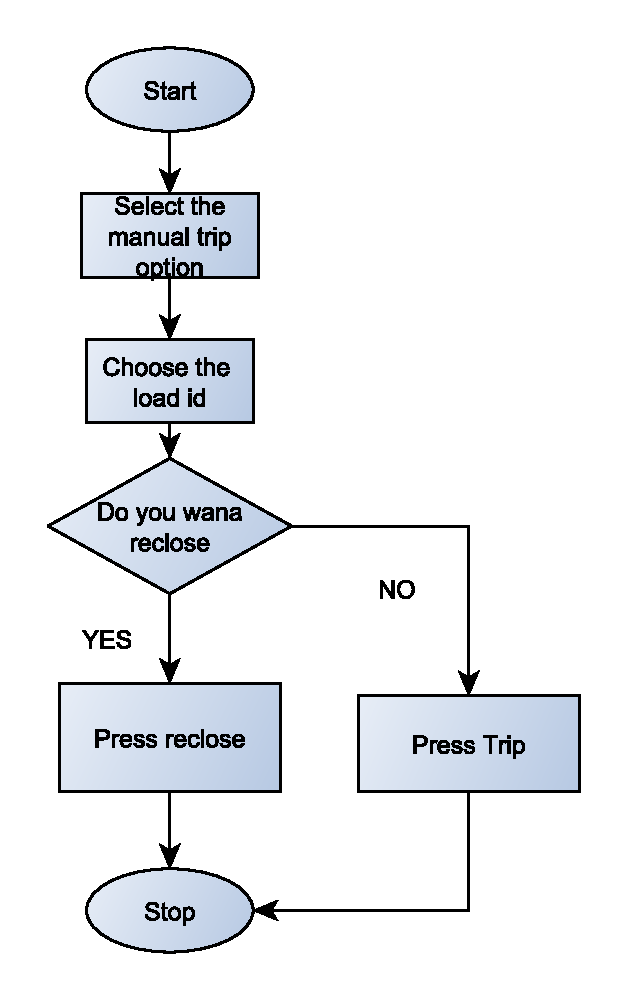
\includegraphics[scale=0.5]{Figures/manualtrip.eps}
		\caption{Flowchart of Manual Controller}
		\label{fig:fcmc1}
	\end{center}
\end{figure}


\paragraph*{Figure} JPEG/JPG Format [Figure \ref{fig:rb}]
\begin{figure}[h]
	\begin{center}
		\includegraphics[scale=0.3]{Figures/relay.jpg}
		\caption{Relay Board}
		\label{fig:rb}
	\end{center}
\end{figure}

\paragraph*{Table} Refer [Table \ref{tab:sm}]
\begin{table}[h]
	\centering
	\caption{Student Marks}
	\begin{tabular}{rr}
		\toprule
		Name  & Marks \\
		\midrule
		Ajay  & 10 \\
		Vinay & 20 \\
		\bottomrule
	\end{tabular}%
	\label{tab:sm}%
\end{table}%


\paragraph*{Cross References: Citation, Index, Reference, Equation reference}
This is the methodology for the entire project work which includes even the process of deciding on the project title, objectives
\index{Ojectives}, etc. This is mandatory for MTech and optional for BTech)\cite{abcdef}. The data is shown in Table \ref{tab:sm}. The equation shown in Equation \eqref{Eq:eq123}

\paragraph*{Inline Equation}
This is my equation.
$	f = ma \pm \alpha \Delta \left[ {\begin{array}{*{20}{c}}
	1 & \chi   \\
	{ - 1} & 0  \\
	\end{array}} \right] $
,which is appearing in between some text.

\paragraph*{Equation without Numbering} 
\begin{equation*}
	x = \frac{{ - b \pm \sqrt {{b^2} - 4ac} }}{{2a}}\
\end{equation*}

\paragraph*{Equation with Numbering} 
\begin{equation} \label{Eq:eq123}
\dot X = \left[ {\begin{array}{*{20}{c}}
	1 & p  \\
	2 & \alpha   \\
	\end{array}} \right]\left[ {\begin{array}{*{20}{c}}
	{{x_1}}  \\
	{{x_2}}  \\
	\end{array}} \right] + Bu\
\end{equation}



\paragraph*{Algorithm Format} 
\begin{algorithm}
	\caption{Addition of two 8 bit numbers}\label{alg:add8bit}
	\begin{algorithmic}[1]	
		\\ Start
		\\ Input a and b
		\\ c=a+b
		\\ Output c
		\\ stop
	\end{algorithmic}
\end{algorithm}


\paragraph*{Enumeration Format}
The following are the different flavor of Tex systems
\begin{enumerate}
	\item TeXLive TeX System
		\begin{enumerate}
			\item TeXLive for Windows
			\begin{enumerate}
				\item TeXLive
				\item ProTex
			\end{enumerate}
			\item MacTeX for Mac
		\end{enumerate}
	\item MikTeX TeX System
\end{enumerate}

\paragraph*{Bullets Format}
The following are the advantages of LaTeX,
\begin{itemize}
	\item {\LaTeX} is highly portable and free.
	\begin{itemize}
		\item Contribute to TUG
		\item Promote Free Softwares
	\end{itemize}
	\item Operating-system independent.
	\item Complex scientific documents can be created
	automatically.
	\item High quality math typesetting.
\end{itemize}

\paragraph*{Program Inclusion} Program file present in other directory can be embedded into the report.
\lstinputlisting{Files/code.asm}

\paragraph*{Verbatim Text} Include text as it is.
\\
The additional database schema is shown below which is used to store all the configuration and transaction data.
\begin{verbatim}
CREATE TABLE `controller_config` (
`load_id` int(11) NOT NULL,
`ct_constant` double DEFAULT NULL,
`pt_constant` double DEFAULT NULL,
`samples` int(11) DEFAULT NULL,
`delay` double DEFAULT NULL,
PRIMARY KEY (`load_id`)
) ENGINE=InnoDB DEFAULT CHARSET=utf8;
SELECT * FROM loadcontroller.load_details;
\end{verbatim} 


 
\chapter{RESULTS, DISCUSSIONS AND CONCLUSIONS} % Main chapter title
\label{ChapterResults} % For referencing the chapter elsewhere, use \ref{Chapter1} 

Here, the results of the project work (literature survey and review along with actual work) shall be listed and discussed in detail with appropriate arguments (result analysis) leading to logical conclusions. The list of conclusions should sync with the project objectives. The scope for future research and development in the field of the current project work must also be included in this chapter. 

\section{Results \& Analysis}

\section{Comparative Study}

\section{Discussions}


\section{Conclusions}
Conclusion should be on new page and the same should come here.


\section{Scope for Future Work}
Future scope should be on new page and the same should come here.



	
	






 

\addtocontents{toc}{\vspace{2em}} % Add a gap in the Contents, for aesthetics



%----------------------------------------------------------------------------------------
%	BIBLIOGRAPHY
%----------------------------------------------------------------------------------------


%\label{Bibliography}

%\lhead{\emph{Bibliography}} % Change the page header to say "Bibliography"

\bibliographystyle{unsrtnat} % Use the "unsrtnat" BibTeX style for formatting the Bibliography
%
%\bibliography{Bibliography} % The references (bibliography) information are stored in the file named "Bibliography.bib"
\addtotoc{BIBLIOGRAPHY}

\begin{thebibliography}{1}

% New edition of a book
\bibitem{BrusawAired}
C. Brusaw, C. Aired, and W. Oliu, \emph{Handbook of Technical Writing}, 3rd ed. New York: St. Martin’s Press, 1987.

\bibitem{abcdef}
S.K. Kenue and J.F. Greenleaf, “Limited angle multifrequency diffiaction tomography,” \emph{IEEE Trans. Sonics Ultrason}., vol. SU-29, no. 6, pp. 213-2 17, July 1982.

% Book
\bibitem{MorseFeshback}
P.M. Morse and H. Feshback, \emph{Methods of Theoretical Physics}. New York: McGraw Hill, 1953.

% Journal Article
\bibitem{KenueGreenleaf}
S.K. Kenue and J.F. Greenleaf, “Limited angle multifrequency diffiaction tomography,” \emph{IEEE Trans. Sonics Ultrason}., vol. SU-29, no. 6, pp. 213-2 17, July 1982.


\bibitem{abcd}
M.M. Botvinnik, \emph{Computers in Chess: Solving Inexact Search Problems}. Translated by A. Brown, Berlin: Springer-Verlap, 1984.

% Article in an Anthology
\bibitem{Broadhead}
G.J. Broadhead, “Style in technical and scientific writing.” In M.G. Moran and D.Joumet, eds. \emph{Research in Technical Communication. A Bibliographic Sourcebook}, pp. 379-401. Westport. CT: Greenwood Press, 1985.

% Translation
\bibitem{Botvinnik}
M.M. Botvinnik, \emph{Computers in Chess: Solving Inexact Search Problems}. Translated by A. Brown, Berlin: Springer-Verlap, 1984.

% Personal Interview/Communication
\bibitem{Elmer}
Interview [or Personal Communication] with Prof. Elmer Hixon, BCE Department, The University of Texas at Austin, March 12, 1995.

% Handbook/date book, no author
\bibitem{Washington}
\emph{Handbook for Writing Operation and Maintenance Manuals.} Washington, D.C.: Packaging Machinery Manufacturers Institute, 1973.

\bibitem{Austin}
\emph{Interface Circuits Data Book}, Texas Instruments, Austin, Texas, 1993.

\bibitem{Microsoft}
\emph{User’s Guide: Microsoft Word,} Vers. 5.0, Microsoft, 1991.

% Encyclopedia Entry

% No author given:
\bibitem{Brittanica}
“Sonar,” \emph{Encyclopaedia Brittanica}, 1984 ed.

% Author(s) given:
\bibitem{PearsonMacChesney}
A.D. Pearson, J.B. MacChesney, and W.G. French, “Fiber optics,” in \emph{Encyclopedia of Semiconductor Technology}, M. Grayson, Ed., New York: John Wiley \& Sons, 1984.

% Online:
\bibitem{BrittanicaOnline}
“Greyhound,” \emph{Brittanica Online}, Beta Version 96.1, March 1996.

% Course Notes
\bibitem{Jones}
J. K. Jones, \emph{Lab Notes for EE464K, Senior Projects}, The University of Texas at Austin, fall semester, 1994.

% Dissertation or thesis
\bibitem{Tsikos}
B. Tsikos, “Segmentation of 3-D scenes using multi-modal interaction between machine vision and programmable mechanical scene manipulation,” Ph.D.
dissertation, Univ. of Pennsylvania, BCE Dept., Philadelphia, 1987.

% Proceedings paper
\bibitem{Finkel}
R. Finkel, R. Taylor, R. Bolles, R. Paul, and J. Feldman, “An overview of AL, programming system for automation,” in \emph{Proc. Fourth Int. Joint Conf Artif. Intell.}, pp. 758-765, Sept. 3-7, 1975.

% Patent
\bibitem{Norman}
L.O. Norman, U.S. Patent 4 379 752, 1983. [Title of patent may be included.]

% Newspaper article
\bibitem{Wall}
“Technology threatens to shatter the world of college textbooks, \emph{The Wall Street Journal}, vol 91, pp. Al, A8, June 1, 1993.

% Government publication
\bibitem{Wall}
\emph{Basic Facts about Patents}. Washington, D.C.: Government Printing Office, 1989.

% Technical Report
\bibitem{CoxTurner}
R. Cox and J. S. Turner, “Project Zeus: design of a broadband network and its
application on a university campus,” Washington Univ., Dept. of Comp. Sci.,
Technical Report WUCS-91-45, July 30, 1991.


% Letter/E-mail
\bibitem{Beck}
Letter from J. M. Beck, Project Manager, TI, Bedford, Utah, Sept. 3, 1996.

% Software
\bibitem{Janzen}
M. Janzen, \emph{Instant Access Accounting}. Computer software. Nexus Software, Inc IBM-PC, 1993.


% Electronic bulletin board
\bibitem{AIDS}
AIDS Info BBS. [San Francisco (CA): Ron Gardner]. Available from: 415-626-1246.

% Database/online
\bibitem{Duncan}
R. Duncan, “An HTML primer,” \emph{PC Magazine}, June 13, 1995, v14, n11 p. 261(7) in Academic Index (database on UTCAT PLUS system).

\bibitem{Berdan}
R. Berdan and M. Garcia, \emph{Discourse-Sensitive Measurement of Language Development in Bilingual Children} (Los Alamitos, CA: National Center for
Bilingual Research, 1982) (ERIC ED 234 636).

% World Wide Web (give author and title if named)
\bibitem{Fuminao}
Fuminao Okumura and Hajime Takagi, “Maglev Guideway On the Yamanashi Test Line,” \emph{http://www.rtri.or.jp/rd/maglev2/okumura.html,} October 24, 1998.

\bibitem{Supplies}
“AT\&T Supplies First CDMA Cellular System in Indonesia,” \emph{http://www.att.com/press/1095/951011.nsa.html}, Feb 5, 1996.

\end{thebibliography}  


%\backmatter
\clearpage % Start a new page

%\chapter{Publication Details}

\publicationlist{
%\label{PublicationDetails}

%\lhead{\emph{Publication Details}}
\justify

S.K. Kenue and J.F. Greenleaf, “Limited angle multifrequency diffiaction tomography,” \emph{IEEE Trans. Sonics Ultrason}., vol. SU-29, no. 6, pp. 213-2 17, July 1982.

}

\pagebreak




%----------------------------------------------------------------------------------------
%	THESIS CONTENT - APPENDICES
%----------------------------------------------------------------------------------------

\addtocontents{toc}{\vspace{2em}} % Add a gap in the Contents, for aesthetics

\appendix % Cue to tell LaTeX that the following 'chapters' are Appendices

% Include the appendices of the thesis as separate files from the Appendices folder
% Uncomment the lines as you write the Appendices

% Appendix A

\chapter{Appendix A Title} % Main appendix title
\label{AppendixA} % For referencing this appendix elsewhere, use \ref{AppendixA}

Since the chapters are numerically numbered, the appendices shall be numbered using alphabets (English capital letters). The items that can be inserted as appendices are (list is not exhaustive):

\begin{itemize}
	\item Project synopsis or proposal (if submitted before starting the project)
	\item Photos
	\item Software model analysis reports (these shall not be inserted in the main body of the report)
	\item Project schedules
	\item Selected material from the data collected
	\item Miscellaneous analysis and reports
\end{itemize}


\section{Appendix A Section 1}

\subsection{Appendix A Subsection for Section 1}

\section{Appendix A Section 2}
% Appendix B

\chapter{Appendix B Title} % Main appendix title
\label{AppendixB} % For referencing this appendix elsewhere, use \ref{AppendixA}


\section{Appendix B Section 1}

\section{Appendix B Section 2}

\section{Appendix B Section 3}




%----------------------------------------------------------------------------------------
%	Index Page
%----------------------------------------------------------------------------------------
\printindex

\end{document}  